\فصل{نتایج عددی}

در این بخش، نتایج آزمایش‌های مونت‌کارلو ارائه می‌شود.  
ابتدا ویژگی CFAR آشکارساز پیشنهادی مورد بررسی قرار می‌گیرد.  
سپس دقت تقریب توزیعی که برای آماره‌ی آشکارساز تحت \لر{SNR}های مختلف به‌دست آورده‌ایم، ارزیابی می‌شود.  
در ادامه، کارایی آشکارساز پیشنهادی با آشکارساز \لر{One-Bit EMR} مقایسه خواهد شد.  
در نهایت نیز تحلیل تئوری ارائه‌شده با نشان دادن اینکه افت کارایی کمتر از $2$ دسی‌بل است، تأیید می‌شود.  

برای تمامی آزمایش‌ها تعداد $10^{6}$ تکرار مونت‌کارلو در نظر گرفته شده است.  
نسبت سیگنال به نویز (SNR) به صورت زیر تعریف می‌شود:
\begin{equation}
	\mathrm{SNR} = 10\log_{10}\!\left(\frac{\bar{\sigma}_{s}^{2}}{\bar{\sigma}_{w}^{2}}\right),
\end{equation}
که در آن $\bar{\sigma}_{s}^{2}=\mathrm{tr}(\mathbf{R}_{s})/p$ و 
$\bar{\sigma}_{w}^{2}=\mathrm{tr}(\mathbf{R}_{w})/m$ هستند.  

\medskip
برای ارزیابی دقت تقریب توزیع‌های به‌دست‌آمده، از معیار \لر{Cramér-von Mises goodness-of-fit} استفاده می‌کنیم.  
این معیار آماری به طور گسترده برای سنجش نزدیکی یک توزیع تقریبی به توزیع واقعی استفاده می‌شود و در حوزه‌هایی نظیر تحلیل داده‌های کلاتر کاربرد فراوان دارد.  

این معیار به صورت زیر تعریف می‌شود:
\begin{equation}
	\epsilon = \frac{1}{K}\sum_{i=1}^{K}\left| F(\xi_{i}) - \hat F(\xi_{i}) \right|^{2},
\end{equation}
که در آن $K$ تعداد آستانه‌های نمونه‌برداری‌شده، $\xi_{i}$ مقدار آستانه‌ی $i$ام، و 
$F(\xi_{i})$ و $\hat F(\xi_{i})$ به‌ترتیب توزیع تجمعی تجربی و توزیع تجمعی تقریبی هستند.  

\قسمت{توزیع \لر{Null}}

ابتدا ویژگی \لر{CFAR} آشکارساز پیشنهادی و نیز آشکارساز \لر{EMR} یک‌بیتی ارزیابی می‌شود. 
پارامترها به صورت $m=4$، $n=128$ و سه سناریوی متفاوت برای واریانس‌های نویز در هر گیرنده در نظر گرفته می‌شوند:
\[
[\sigma_{w1}^{2},\sigma_{w2}^{2},\sigma_{w3}^{2},\sigma_{w4}^{2}]
\in \big\{[1,1,1,1],~[0.4,\,0.8,\,1.2,\,1.6],~[0.5,\,0.75,\,1.2,\,1.5]\big\}.
\]
\textbf{توجه:} در متن مقاله به‌اشتباه نماد $\sigma_{wi}$ (بدون توان دو) برای این مقادیر آمده است، 
اما از آن‌جا که این مقادیر مستقیماً به‌عنوان درایه‌های قطری $\mathbf{R}_{w}$ (ماتریس کوواریانس نویز) استفاده می‌شوند، 
باید آن‌ها را واریانس در نظر گرفت. 

\begin{figure}[!b]
	\centering
	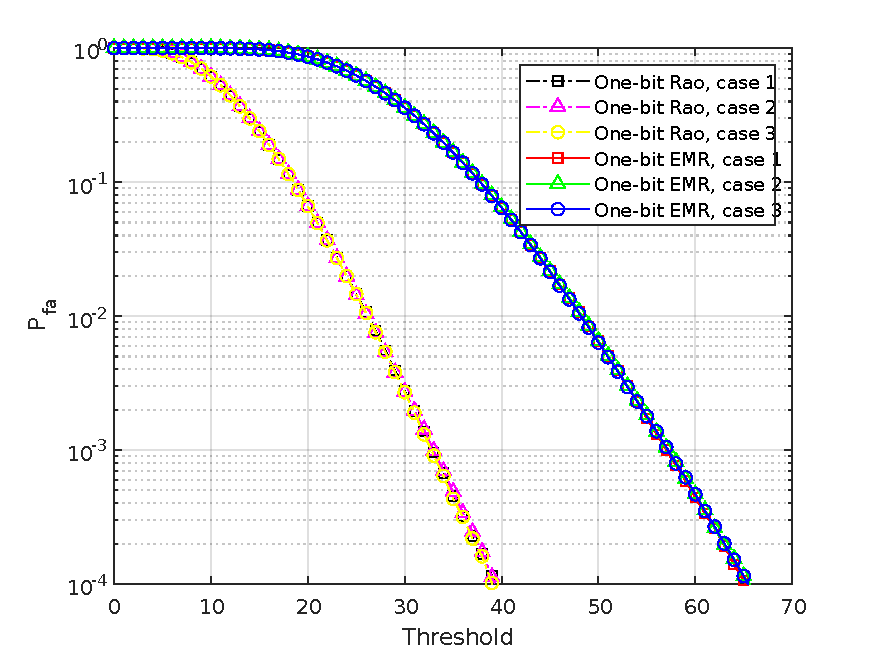
\includegraphics[width=0.8\linewidth]{figs/cfar}
	\caption[احتمال \lr{false alarm} بر حسب آستانه]{
	احتمال \لر{false alarm} برحسب آستانه برای 
	$m=4$
	و
	$n=128$
	و سه حالت \لر{case1}، \لر{case2} و \لر{case3} که به ترتیب متناظر با مقادیر
	$
	[1,1,1,1]$,~$[0.4,\,0.8,\,1.2,\,1.6]$
	و ~$[0.5,\,0.75,\,1.2,\,1.5]$
	برای
	$[\sigma_{w1}^{2},\sigma_{w2}^{2},\sigma_{w3}^{2},\sigma_{w4}^{2}]$
	هستند
	}
	\label{fig:CFAR}
\end{figure} 

نتایج در شکل~\ref{fig:CFAR} (شکل~1 مقاله) نمایش داده شده‌اند.
برای آن‌که خروجی آزمون \لر{EMR} یک‌بیتی و آشکارساز پیشنهادی در یک بازهٔ مشابه قرار گیرند، 
آمارۀ \لر{EMR} یک‌بیتی مطابق
\[
T_{O}' \;=\; m n \big(T_{O}-1\big)
\]
مقیاس‌بندی می‌شود. 
شکل~\ref{fig:CFAR} نشان می‌دهد هر دو آشکارساز دارای خاصیت \لر{CFAR} هستند که با نتایج تحلیلی بخش‌های قبلی سازگار است.

\begin{figure}[!t]
	\centering
	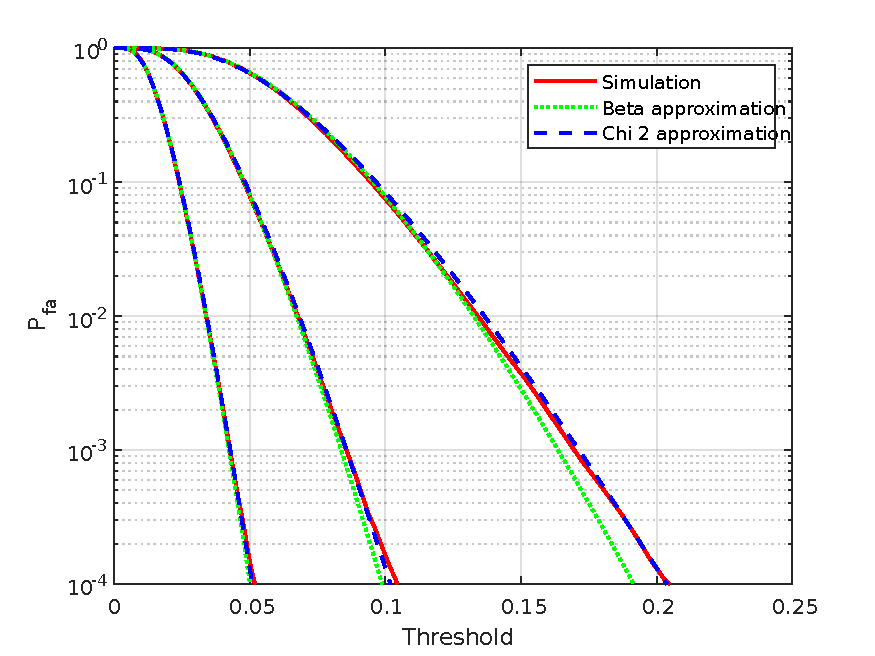
\includegraphics[width=0.8\linewidth]{figs/false_alarm}
	\caption[احتمال \lr{false alarm} بر حسب آستانه برای $n$ های مختلف]{
		احتمال \لر{false alarm} برحسب آستانه برای 
		$m=4$
		و
		$n=16,32,64$
	}
	\label{fig:false_alarm}
\end{figure} 




\medskip
در ادامه، دقت توزیع‌های نالِ (تحت $H_{0}$) آشکارساز پیشنهادی بررسی می‌شود. توزیع‌های تقریبی مورد مقایسه، \eqref{eq:beta_approx} و \eqref{eq:chi_approx} هستند.
نتایج شبیه‌سازی در شکل~\ref{fig:false_alarm} (شکل~2 مقاله) آمده است. 
برای این بخش $m=4$ و $n\in\{16,\,32,\,64\}$ در نظر گرفته می‌شود. 
\emph{توجه شود} که از آمارۀ نرمالیزه‌شدهٔ $T_{R}'$ تعریف‌شده در رابطهٔ \eqref{eq:TRPrime} استفاده می‌کنیم، 
زیرا $T_{R}'\in[0,1]$ است. 
به‌طور هم‌زمان، نتیجهٔ رابطهٔ \eqref{eq:chi_approx} نیز با تعریف
\[
\gamma' \;=\; \frac{\gamma}{m n (m-1)}
\]
نرمالیزه می‌شود.

شکل~\ref{fig:false_alarm} نشان می‌دهد که برای $n=16$، هر دو توزیعِ بتا و $\chi^{2}$ در مقادیر بزرگ $P_{fa}$ 
برازش خوبی نسبت به توزیع تجربی دارند، 
در حالی‌که توزیع $\chi^{2}$ در مقادیر کوچک $P_{fa}$ برازش بهتری ارائه می‌کند. 
با افزایش $n$، هر دو تقریبِ بتا و $\chi^{2}$ به‌تدریج به توزیع تجربی نزدیک‌تر می‌شوند و برای $n=64$ 
برازش رضایت‌بخشی حاصل می‌گردد. 
\begin{table}[t]
	\centering
	\caption{خطای توزیع‌های تقریبی نال}
	\label{tab:null_error}
	\begin{tabular}{cccc}
		\hline
		\multicolumn{4}{c}{$m=4$} \\ \hline
		تقریب 
		& $n=16$ & $n=32$ & $n=64$ \\ \hline
		بتا
		& \lr{9.9863e-06} & \lr{2.4253e-06} & \lr{7.4587e-07} \\ \hline
		کای-دو
		& \lr{1.5484e-05} & \lr{3.531e-06} & \lr{9.8966e-07} \\ \hline
	\end{tabular}
\end{table}
این مشاهده با خطای تقریبی گزارش‌شده در جدول \ref{tab:null_error} توصیف می‌شود؛ 
این جدول نشان می‌دهد \emph{به‌طور کلی} توزیع بتا نسبت به $\chi^{2}$ برازش کلی بهتری ارائه می‌دهد.
\قسمت{توزیع \لر{Non-Null}}

در این بخش، دقت تقریب‌های توزیع نان‌نال (تحت $H_{1}$) برای آشکارساز پیشنهادی بررسی می‌شود.  
تقریب‌های مورد مقایسه روابط \eqref{eq:beta_approx2} و \eqref{eq:chi_approx} هستند.  
پارامترها به صورت $m=4$، $p=2$، $n=\{64,128,256\}$ و 
$\mathrm{SNR}=\{-9~\mathrm{dB},\,4~\mathrm{dB}\}$ تنظیم شده‌اند.  
برای افزایش قابلیت بازتولید نتایج، ماتریس کانال به‌صورت زیر مشخص شده است:
\[
\mathbf{H}=
\begin{bmatrix}
	0.5282 - j\,0.0658 & -0.3370 - j\,0.4516 \\
	0.0294 + j\,0.3040 &  0.7462 + j\,0.1550 \\
	-0.5102 - j\,0.2616 & -0.1954 - j\,0.0563 \\
	-0.2539 - j\,0.4797 &  0.2375 - j\,0.0622
\end{bmatrix}.
\]

\begin{figure}[!b]
	\centering
	\subfigure[$SNR=-9dB$]{
		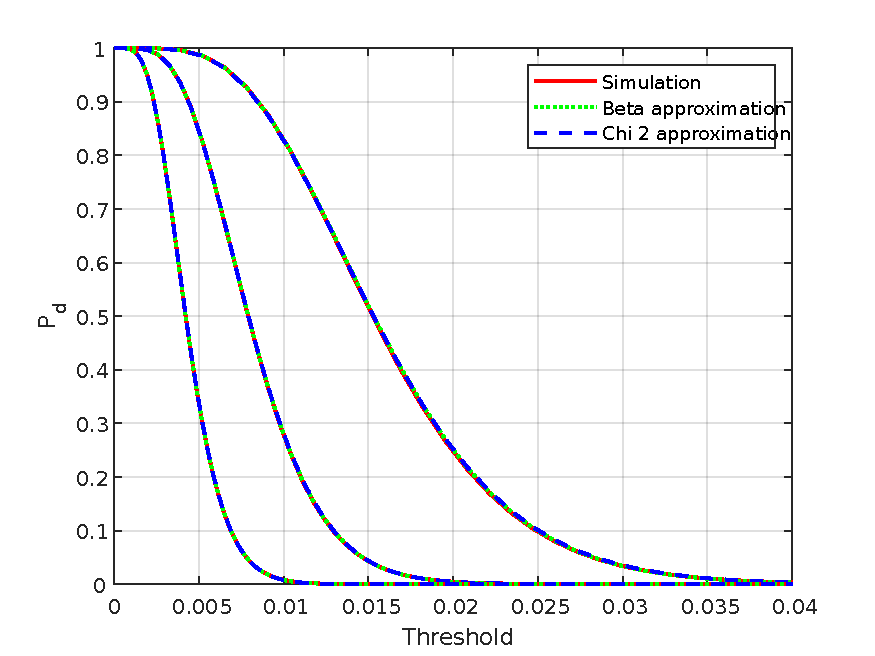
\includegraphics[width=0.8\linewidth]{figs/detection_SNR-9}
	} \\
	\subfigure[$SNR=4dB$]{
		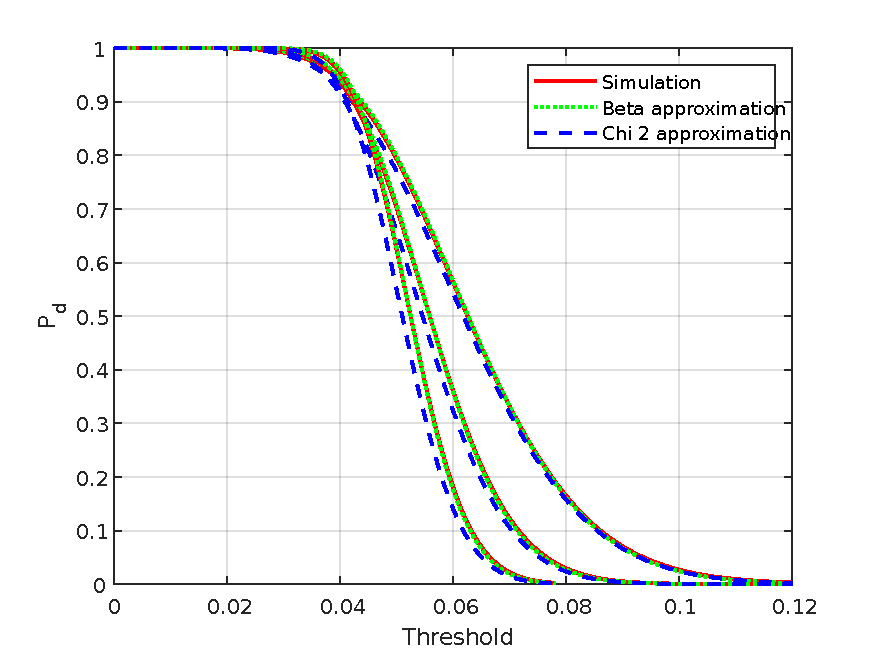
\includegraphics[width=0.8\linewidth]{figs/detection_SNR4}
	}
	\caption[
	احتمال آشکارسازی برحسب آستانه
	]{
	احتمال آشکارسازی برحسب آستانه برای
	 $m=4$، $p=2$ و
	 $n=64,128,256$
	}
	\label{fig:detection}
\end{figure}


شکل~\ref{fig:detection} نتایج را نشان می‌دهد.  
در شکل \ref{fig:detection}(آ) (سناریوی SNR پایین)، هر دو تقریب برازش بسیار خوبی با توزیع تجربی دارند.  
در مقابل، \ref{fig:detection}(ب) (سناریوی SNR بالا) نشان می‌دهد که توزیع بتا، همچنان دقت مناسبی در برازش دارد، 
در حالی که توزیع $\chi^{2}$ غیرمرکزی، دقت رضایت‌بخشی ندارد.  


\begin{table}[t]
	\centering
	\caption{خطای توزیع‌های تقریبی نان‌نال}
	\label{tab:non_null_error}
	\begin{tabular}{ccccccc}
		\hline
		\! & \multicolumn{3}{c}{$SNR=-9dB, m=4, p=2$} & \multicolumn{3}{c}{$SNR=4dB, m=4, p=2$} \\ \hline
		تقریب 
		& $n=64$ & $n=128$ & $n=256$ & $n=64$ & $n=128$ & $n=256$ \\ \hline
		بتا
		& \lr{1.1732e-06} & \lr{1.8868e-07} & \lr{5.2847e-087}
		& \lr{2.7991e-06} & \lr{5.95e-06} & \lr{8.2032e-06} \\ \hline
		کای-دو
		& \lr{1.4744e-06} & \lr{3.155e-07} & \lr{1.969e-07} 
		& \lr{4.5341e-05} & \lr{0.00026271} & \lr{0.0010241} \\ \hline
	\end{tabular}
\end{table}

این نتایج با خطاهای تقریبی گزارش‌شده در جدول \ref{tab:non_null_error} نیز توصیف می‌شود.
این جدول نشان می‌دهد که برای SNR پایین، هر دو تقریب دقت بالایی دارند، 
اما در SNR بالا تنها تقریب بتا قادر به برازش مناسب است.  
علت این تفاوت آن است که توزیع بتا با روش ممان‌ها \لر{(method of moments)} به‌دست آمده و محدودیتی روی مقدار SNR ندارد، 
در حالی که توزیع $\chi^{2}$ غیرمرکزی، تحت فرض SNR پایین استخراج شده است؛
از این رو در SNR بالا دقت خود را از دست می‌دهد.

\قسمت{عملکرد آشکارسازی}

در این شبیه‌سازی، کارایی آشکارساز پیشنهادی با تست \لر{EMR} یک‌بیتی از طریق منحنی‌های \emph{ROC} مقایسه می‌شود.  

پارامترها به صورت $m=4$، $p=2$، $n=128$ و $\mathrm{SNR}=-1~\mathrm{dB}$ در نظر گرفته شده‌اند.  
ماتریس کانال $\mathbf{H}$ همان مقدار بخش قبلی انتخاب می‌شود.  

همچنین، برای بررسی اثر کالیبراسیون گیرنده، دو مجموعه‌ی متفاوت از واریانس‌های نویز به کار گرفته می‌شوند:  
\begin{itemize}
	\item در سناریوی اول، واریانس نویز همه‌ی گیرنده‌ها برابر با $1$ در نظر گرفته می‌شود.  
	\item در سناریوی دوم، واریانس‌ها به صورت 
	\([\,\sigma_{w1}^{2},\,\sigma_{w2}^{2},\,\sigma_{w3}^{2},\,\sigma_{w4}^{2}\,] 
	= [0.4,\,0.8,\,1.2,\,1.6]\) تنظیم می‌شوند،  
	به‌طوری که توان کل نویز در هر دو حالت ثابت باقی می‌ماند.  
\end{itemize}

\begin{figure}[!b]
	\centering
	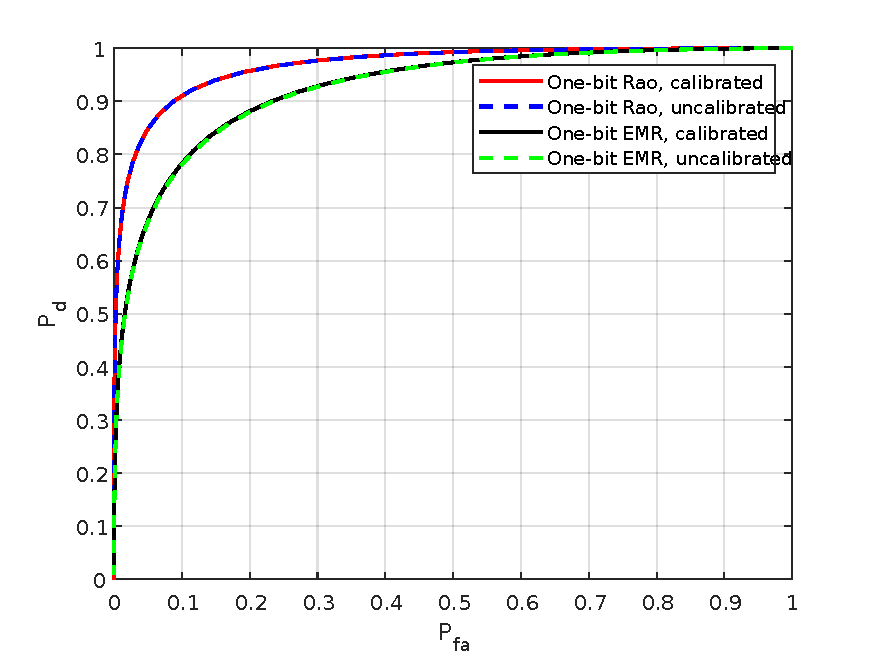
\includegraphics[width=0.8\linewidth]{figs/roc}
	\caption[
	\لر{ROC}های تجربی
	]{
		\لر{ROC}های تجربی به دست آمده برای
		$m=4$, $p=2$, $n=128$ و
		$SNR=-1dB$
	}
	\label{fig:ROC}
\end{figure} 

نتایج در شکل~\ref{fig:ROC} (شکل ۴ مقاله) نشان داده شده‌اند.  
این نتایج بیانگر آن است که روش پیشنهادی عملکرد بهتری نسبت به آشکارساز \لر{EMR} یک‌بیتی دارد.  
علاوه بر این، قابل توجه است که کارایی هر دو آشکارساز (\لر{EMR} و روش پیشنهادی) 
در حالت‌های کالیبره و غیرکالیبره یکسان باقی می‌ماند.  



\قسمت{افت کارایی}

در این بخش، شکاف کارایی بین آشکارساز پیشنهادی یک‌بیتی و آشکارسازهای $\infty$-بیتی بررسی می‌شود.  
برای این منظور، احتمال \لر{false alarm} روی مقدار ثابت $P_{fa}=10^{-4}$ نگه داشته شده و سپس تغییرات احتمال آشکارسازی نسبت به SNR بررسی می‌گردد.  

پارامترها به صورت $m=4$، $p=2$ و $n\in\{128,\,2048\}$ انتخاب شده‌اند.  
برای لحاظ کردن اثر احتمالی انتخاب ماتریس کانال $\mathbf{H}$ بر عملکرد آشکارسازی، از یک روش \emph{میانگین‌گیری وزنی} استفاده می‌شود؛  
به‌طور مشخص، در هر اجرای آزمایش، ماتریس $\mathbf{H}$ به‌طور تصادفی از یک توزیع گوسی مختلط دایره‌ای با میانگین صفر (ZMCSCG) تولید و سپس ستون‌های آن نرمالیزه می‌شوند.  

نتایج در شکل~\ref{fig:detection_diff_n} (شکل~5 مقاله) نشان داده شده‌اند.  
از این نتایج می‌توان مشاهده کرد که، با تعداد نمونه‌ی یکسان، افت کارایی آشکارساز پیشنهادی نسبت به آشکارساز $\mathrm{EMR}$ یک‌بیتی کمتر است.  
افزون بر این، \ref{fig:detection_diff_n}(آ) نشان می‌دهد که وقتی $n$ به اندازه‌ی کافی بزرگ نباشد، شکاف کارایی بین آشکارساز پیشنهادی و آزمون LMPIT بیش از $2$ دسی‌بل است.  
در مقابل، \ref{fig:detection_diff_n}(ب) نشان می‌دهد که در SNR پایین و با $n$ بزرگ، افت کارایی آشکارساز پیشنهادی نسبت به LMPIT تقریباً برابر با $2$ دسی‌بل است.  
این مشاهده با نتایج تحلیلی بخش‌های قبل سازگار است .  

همچنین، با کاهش SNR شکاف کارایی بین آشکارساز پیشنهادی و تست $\infty$-بیتی EMR نیز کاهش می‌یابد، اگرچه همچنان اندکی بالاتر از $2$ دسی‌بل باقی می‌ماند.  
علت این موضوع آن است که تست $\infty$-بیتی EMR علاوه بر استقلال، برابری واریانس‌های نویز را نیز در نظر می‌گیرد، در حالی‌که در حالت یک‌بیتی با از دست رفتن اطلاعات دامنه، این ویژگی دیگر نقشی در توان آشکارسازی ندارد و موجب افزایش اندک افت کارایی می‌شود .  

شکل \ref{fig:detection_diff_n} همچنین نشان می‌دهد که وقتی تعداد نمونه‌ها حدود $2.47n$ برابر افزایش یابد، منحنی عملکرد آشکارساز پیشنهادی با منحنی آزمون LMPIT به‌طور کامل هم‌پوشانی پیدا می‌کند.  
به‌ویژه، در شکل \ref{fig:detection_diff_n}(آ) بین منحنی آشکارساز پیشنهادی و LMPIT شکاف ۲ دسی‌بل وجود دارد، در حالی‌که آشکارساز پیشنهادی با $2.47n$ نمونه دقیقاً با منحنی LMPIT هم‌راستا می‌شود.  
این نتیجه اهمیت کلیدی افزایش اندازه‌ی نمونه‌ها را در صحت چارچوب تحلیلی ارائه‌شده در رابطه‌ی \eqref{eq:chi_approx} نشان می‌دهد.

\begin{figure}[!b]
	\centering
	\subfigure[$n=128$]{
		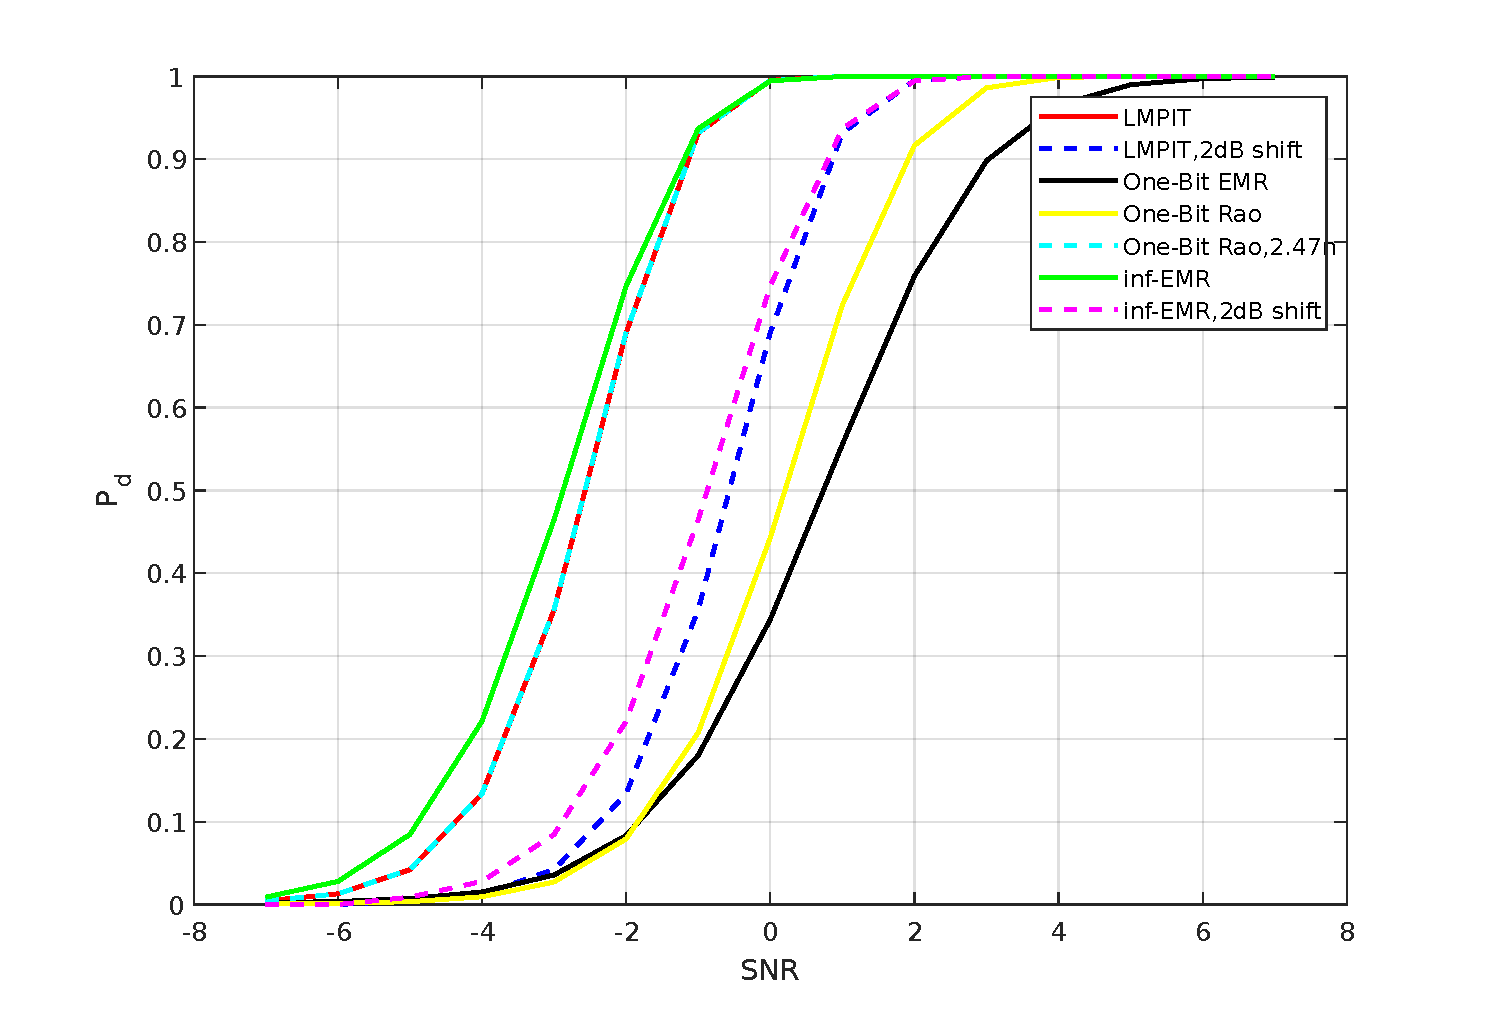
\includegraphics[width=0.8\linewidth]{figs/detection128}
	} \\
	\subfigure[$n=2048$]{
		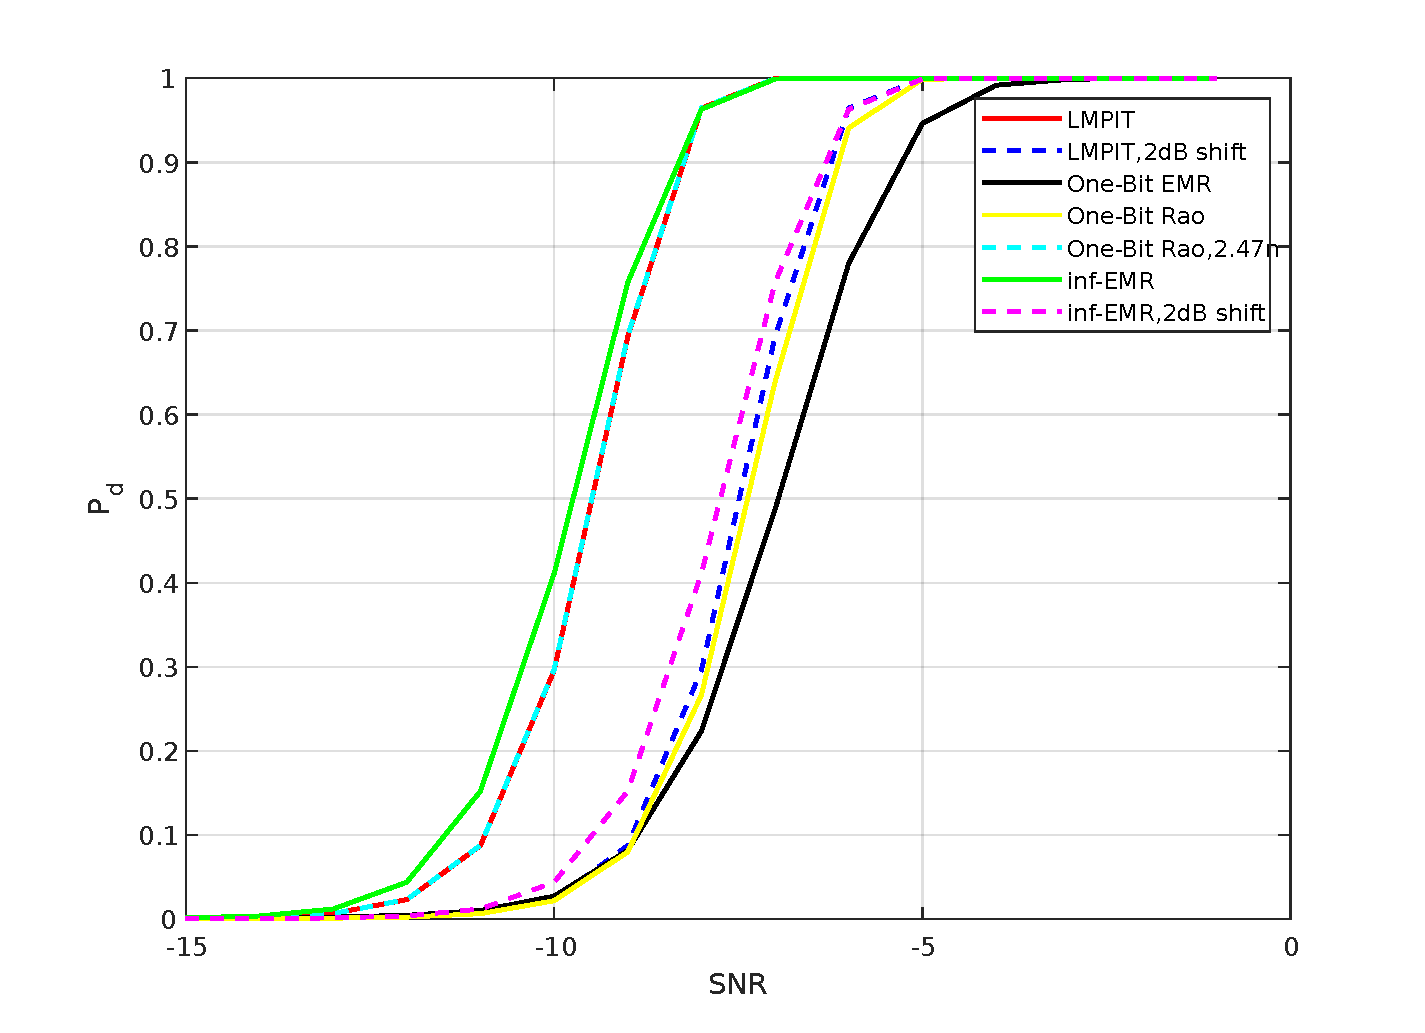
\includegraphics[width=0.8\linewidth]{figs/detection2048}
	}
	\caption[
	احتمال آشکارسازی برحسب \لر{SNR}
	]{
		احتمال آشکارسازی برحسب \لر{SNR} برای
		$m=4$، $p=2$ و
		$P_{fa}=10^{-4}$
	}
	\label{fig:detection_diff_n}
\end{figure}
